\documentclass[fontsize=12pt,paper=a4,twoside]{scrartcl}

% Dokumentenpräambel
% hier alle Packages die genutzt werden mittels \usepackage einbinden
\usepackage{booktabs}

\usepackage[utf8]{inputenc}

\usepackage[final]{pdfpages}

\usepackage[ngerman]{babel} 

% für Deutschunterstützung und neue Rechtschreibung
\usepackage[ngerman]{varioref} 

% Verweise innerhalb des Dokuments schick mit " ... auf Seite ... " automatisch versehen. Dazu \vref{labelname} benutzen
\usepackage{ngerman}

% obere Seitenränder gestalten können
\usepackage{fancyhdr}

% Graphiken als jpg, png etc. einbinden können
\usepackage{graphicx}

% Unterstützung für etliche Symbole
\usepackage{stmaryrd}

% Floats Objekte mit [H] festsetzen
\usepackage{float}

% setzt URL's schön mit \url{http://bla.laber.com/~mypage}
\usepackage{url}

% Externe PDF's einbinden können
\usepackage{pdflscape}

% Bibliographie
\usepackage{bibgerm}

% Tabellen
\usepackage{tabularx}

\usepackage{supertabular}

\usepackage[colorlinks=true, pdfstartview=FitV, linkcolor=blue, citecolor=blue, urlcolor=blue, hyperfigures=true, pdftex=true]{hyperref}

\usepackage{bookmark}

%
% hier Formatierungsbefehle einfügen
%
% Damit Latex nicht zu lange Zeilen produziert
\sloppy

% Uneinheitlicher unterer Seitenrand
\raggedbottom

% Pfad zu den Grafiken fürs Dokument. Ordner muss im gleichen Verzeichniss liegen
\graphicspath{{graphics/},{graphics/ScreensWebsite/}}

% Gafikendungen die genutzt werden
\DeclareGraphicsExtensions{.png,.jpg}

% Seitenränder für Korrekturen setzen
\addtolength{\evensidemargin}{-1cm}\addtolength{\oddsidemargin}{1cm}

% Kein Erstzeileneinzug beim Absatzanfang. Sieht nur gut aus, wenn man zwischen Absätzen viel Platz einbaut.
\setlength{\parindent}{0ex} 

% Abstand zwischen zwei Absätzen
\setlength{\parskip}{1ex}

% hier werden neue Befehle deklariert
% Header für alle Seiten
\pagestyle{fancy} \setlength{ 
\headheight}{70.55003pt} \fancyhead{} \fancyhead[LO,RE]{Software-Projekt 2\\
2013/14 \\Architekturbeschreibung} \fancyhead[LE,RO]{Seite \thepage\\\slshape \leftmark\\
\slshape\rightmark}

%
% Ab hier beginnt das Dokument
%
\begin{document}

% Lustige Header nur auf dieser Seite
\thispagestyle{fancy} \fancyhead[LO,RE]{ } \fancyhead[LE,RO]{Universität Bremen\\FB 3 -- Informatik\\
Prof. Dr. Rainer Koschke \\TutorIn: Sabrina Wilske} \fancyfoot[C]{}

% Start Titelseite
\vspace{3cm} 
\begin{minipage}
	[H]{ 
	\textwidth} 
	\begin{center}
		\bf \Large Software-Projekt 2 2013/14\\
		\smallskip \small VAK 03-BA-901.02\\
		\vspace{3cm} 
	\end{center}
\end{minipage}
\begin{minipage}
	[H]{ 
	\textwidth} 
	\begin{center}
		\vspace{1cm} \bf \Large Architekturbeschreibung\\
		\vspace{3ex} \small IT\_R3V0LUT10N\\
		\vfill 
	\end{center}
\end{minipage}
\vfill 
\begin{minipage}
	[H]{ 
	\textwidth} 
	\begin{center}
		\sf 
		\begin{tabular}
			{lrr} Sebastian Bredehöft & sbrede@tzi.de & 2751589\\
			Patrick Damrow & damsen@tzi.de & 2056170\\
			Tobias Dellert & tode@tzi.de & 2936941\\
			Tim Ellhoff & tellhoff@tzi.de & 2520913\\
			Daniel Pupat & dpupat@tzi.de & 2703053\\
		\end{tabular}
		\\
		~ \vspace{2cm} \\
		\it Abgabe: 22. Dezember 2013 -- Version 1.7 vom 19.12.2013 \\
		~ 
	\end{center}
\end{minipage}

% Ende Titelseite
% Eine Leerseite
\newpage

\thispagestyle{fancy} \fancyhead{} \fancyhead[LO,RE]{Software-Projekt 2 \\
2013/14 \\Architekturbeschreibung} \fancyhead[LE,RO]{Seite \thepage\\\slshape \leftmark\\~} \fancyfoot{} 
\renewcommand{\headrulewidth}{0.4pt} 
\tableofcontents
\newpage
% Abbildungsverzeichnis 
\listoffigures

% Tabellenverzeichnis
\listoftables

\clearpage

\fancyhead[LE,RO]{Seite \thepage\\
\slshape \leftmark\\
\slshape\rightmark}
%%%%%%%%%%%%%%%%%%%%%%%%%%%%%%%%%%%%%%%%%%%%%%%%%%%%%%%%%%%%%%%%%%%%%%%%
\section*{Version und Änderungsgeschichte}

\begin{tabular}{ccl}
Version & Datum & Änderungen \\
\hline
1.0 & 25.11.2013 & Dokumentvorlage als initiale Fassung kopiert \\
1.1 & 07.12.2013 & Einführung \\
1.2 & 08.12.2013 & Globale Analyse \\
1.3 & 12.12.2013 & Ausführungssicht \\
1.4 & 15.12.2013 & Konzeptionelle Sicht \\
1.5 & 18.12.2013 & Modulsicht u. Datensicht \\
1.6 & 19.12.2013 & Zusammenhänge zwischen Anwendungsfällen und Architektur\\
1.7 & 19.12.2013 & Evolution \\
\end{tabular}


%%%%%%%%%%%%%%%%%%%%%%%%%%%%%%%%%%%%%%%%%%%%%%%%%%%%%%%%%%%%%%%%%%%%%%%%
\section{Einführung (Patrick)}

\subsection{Zweck}

Dieses Dokument ist die Architekturbeschreibung der von uns zu entwickelnden Software. Sie dient der Kommunikation zwischen allen Interessenten. Dies ist unerlässlich für die Entwicklung des Systems, da die Entwickler der Architekturbeschreibung die Funktionalität einzelner Komponenten entnehmen. Sie dient der Aufteilung der Arbeit in unabhängig bearbeitbare Teile, besitzt anfangs einen hohen Abstraktionsgrad, der von vielen verstanden werden kann und wird in den Schichten weiter unten in diesem Dokument präziser ausgearbeitet. Die präzise Ausarbeitung der Architektur ist wichtig, um Möglichkeiten und Probleme der Entwicklung auszuloten und präventive Strategien und Maßnahmen zu entwickeln.

Die Architektur des Systems ist daher das Fundament unserer Implementierung, die direkt aus der Architektur resultiert.


\subsection{Status}

Dies ist der erste Architekturentwurf vom 22.12.2013.
\subsection{Definitionen, Akronyme und Abkürzungen}

\subsection{Referenzen}

\begin{itemize}
	\item{\url{http://www.informatik.uni-bremen.de/st/Lehre/swpII_1314/mindestanforderungen.html}\\
	Die Mindestanforderungen für das Produkt.}
	\item{\url{http://www.elearning.uni-bremen.de} Plattform der Universität Bremen. Zugriff auf Folien der Veranstaltung Software Projekt 1 des Sommersemesters 2013 und Übungen des Software Projekts 2 des Wintersemesters 13/14 nur eingeschränkt möglich.} 
	\item{Vorlage dieses Dokuments - Stud.IP Software Projekt 2\\
	 3-Architekturbeschreibung-Vorlage.tex} 
	\item{Hinweise zu diesem Dokument - Stud.IP 3-Hinweise-Abgabe-Architektur.pdf} 
	\item{\url{http://www.informatik.uni-bremen.de/st/lehre/swp0809/anette_architekturbeschreibung.pdf}} Architekturbeschreibung einer Gruppe aus dem Software-Projekt 08/09 der Universität Bremen.
\end{itemize}
\subsection{Übersicht über das Dokument}

Dieses Dokument basiert auf der Vorlage des \textit{IEEE P1471 2002} Standards. Der Inhalt dieses Dokuments ist wie folgt aufgegliedert:

\begin{enumerate}
\item{\textbf{Einführung}}

Die Einführung beschreibt den Nutzen dieses Dokuments. Sie erläutert Definitionen, Akronyme und Abkürzungen und listet die benutzten Referenzen auf, sowie eine Übersicht über dieses Dokument.

\item{\textbf{Globale Analyse}}

In diesem Abschnitt werden die relevanten Einflussfaktoren aufgezeigt und bewertet, sowie Strategien entwickelt, um Probleme bzw. interferierende Einflussfaktoren zu behandeln und auf diese entsprechend zu reagieren.

\item{\textbf{Konzeptionelle Sicht}}

Die konzeptionelle Sicht zeigt grob die einzelnen Komponenten und deren Zusammenspiel des zu entwickelnden Systems auf. Dies geschieht auf einer hohen Abstraktionsebene und wird im weiteren Verlauf des Dokuments und den folgenden Sichten konkretisiert und verfeinert.

\item{\textbf{Modulsicht}}

Im Abschnitt Modulsicht dieser Architekturbeschreibung geht es um eine tiefere Ebene der Abstraktion. Hier werden die Komponenten in einzelne Pakete zerlegt und diese wiederum in Module, welche eine Einheit bilden, die ein Entwickler in einer Arbeitswoche implementieren kann.

\item{\textbf{Datensicht}}

Die Datensicht beschreibt das zugrundeliegende Datenmodell und das Zusammenspiel der einzelnen Daten der Datenbank. Dies wird in Form eines erklärenden Textes und UML-Diagrammen realisiert.

\item{\textbf{Ausführungssicht}}

Die Ausführungssicht zeigt im Prinzip das System in ''Aktion'', d.h. es zeigt auf, welche Prozesse laufen, welche Module hierfür gebraucht werden und wie diese zusammenspielen.

\item{\textbf{Zusammenhänge zwischen Anwendungsfällen und Architektur}}

Hier werden die Zusammenhänge zwischen Architektur und den Anwendungsfällen der Anforderungsspezifikation beschrieben.

\item{\textbf{Evolutoin}}

In diesem Teil der Architekturbeschreibung wird beschrieben, welche Änderungen vorgenommen werden müssen, wenn sich Anforderungen und oder Rahmenbedingungen ändern. Ein besonderes Augenmerk liegt hierbei auf die in der Anforderungsspezifikation unter ''Ausblick'' genannten Punkte.

\end{enumerate}

\section{Globale Analyse (Daniel)}
\label{sec:globale_analyse}

\subsection{Einflussfaktoren}
\label{sec:einflussfaktoren}

Die Einflussfaktoren werden im Folgenden unterteilt in:

\begin{itemize}
\item{Organisatorische Faktoren}
\item{Technische Faktoren}
\item{Produktfaktoren}
\end{itemize}

\subsubsection{Organisatorische Faktoren}
\label{sec:orgfaktoren}

\begin{table}[H]
\centering
\caption{Organisatorische Faktoren}
\begin{tabular}{|l|l|} \hline
\textbf{O1} & \textbf{Time-To-Market} \\ \hline
\textbf{O2} & \textbf{Auslieferung von Produktfunktionen} \\ \hline
\textbf{O3} & \textbf{Budget} \\ \hline
\textbf{O4} & \textbf{Kenntnisse in Java und Android} \\ \hline
\textbf{O5} & \textbf{Kenntnisse in J-Unit} \\ \hline
\textbf{O6} & \textbf{Anzahl der Entwickler}\\ \hline
\end{tabular}
\end{table}

\begin{table}[H]
\caption{O1}
\begin{tabular}{|p{3cm}|p{12cm}|}\hline
\textbf{O1} & \textbf{Time-To-Market}\\ \hline \hline
Faktor & Auslieferungsdatum 23.02.2014\\ \hline
Flexibilität und Veränderlichkeit & Die Deadline kann nicht verändert werden.\\ \hline
Auswirkungen & Die Software muss zum Abgabedatum lauffähig sein.\\ \hline
\end{tabular}
\end{table}

\begin{table}[H]
\caption{O2}
\begin{tabular}{|p{3cm}|p{12cm}|}\hline
\textbf{O2} & \textbf{Auslieferung von Produktfunktionen}\\ \hline \hline
Faktor & Alle Mindestanforderungen\\ \hline
Flexibilität und Veränderlichkeit & Es müssen alle Mindestanforderungen erfüllt sein; sie sind jedoch vom Kunden oder beim Verlassen eines Gruppenmitglieds veränderbar.\\ \hline
Auswirkungen & Architektur muss alle Mindestanforderungen abdecken; es muss darauf geachtet werden, dass diese sich im Verlauf noch ändern.\\ \hline
\end{tabular}
\end{table}

\begin{table}[H]
\caption{O3}
\begin{tabular}{|p{3cm}|p{12cm}|}\hline
\textbf{O3} & \textbf{Budget} \\ \hline \hline
Faktor & Kein finanzielles Budget\\ \hline
Flexibilität und Veränderlichkeit & Es werden keine finanziellen Unterstützungen für das Produkt geben. \\ \hline
Auswirkungen & Es können keine kostenpflichtigen Dienste in Anspruch genommen werden.\\ \hline
\end{tabular}
\end{table}

\begin{table}[H]
\caption{O4}
\begin{tabular}{|p{3cm}|p{12cm}|}\hline
\textbf{O4} & \textbf{Kenntnisse in Java und Android} \\ \hline \hline
Faktor & Kenntnisse der Entwickler in Java und Android\\ \hline
Flexibilität und Veränderlichkeit & Kenntnisse sind nicht flexibel, es muss in Java programmiert werden und über Smartphone laufen. Die Kenntnisse können sich im Laufe ändern, z.B. durch neue Erfahrungen und neu erworbene Kenntnisse.\\ \hline
Auswirkungen & Bei wenig Kenntnissen muss mehr Zeit eingeplant werden, um sich diese anzueignen.\\ \hline
\end{tabular}
\end{table}

\begin{table}[H]
\caption{O5}
\begin{tabular}{|p{3cm}|p{12cm}|}\hline
\textbf{O5} & \textbf{Kenntnisse in J-Unit} \\ \hline \hline
Faktor & Kenntnisse in J-Unit Tests\\ \hline
Flexibilität und Veränderlichkeit & Da Tests mit J-Unit gefordert werden, sind diese nicht verhandelbar oder flexibel.\\ \hline
Auswirkungen & Bei unzureichenden Tests kann es später beim Programm zu Problemen kommen, da Fehler spät oder gar nicht erkannt werden.\\ \hline
\end{tabular}
\end{table}

\begin{table}[H]
\caption{O6}
\begin{tabular}{|p{3cm}|p{12cm}|}\hline
\textbf{O6} & \textbf{Anzahl der Entwickler}\\ \hline \hline
Faktor & Die Anzahl der Entwickler\\ \hline
Flexibilität und Veränderlichkeit & Es können keine neuen Gruppenmitglieder dazukommen, es können aber jederzeit Gruppenmitglieder wegfallen. \\ \hline
Auswirkungen & Wenn Gruppenmitglieder wegfallen, müssen die restlichen Mitglieder mehr Arbeit und mehr Zeit einplanen. Auch müssen Projektplan und Architektur neu angepasst werden.\\ \hline
\end{tabular}
\end{table}

\subsubsection{Technische Faktoren}
\label{sec:techfaktoren}

\begin{table}[H]
\centering
\caption{Technische Faktoren}
\begin{tabular}{|l|l|} \hline
\textbf{T1} & \textbf{Software funktioniert unter Windows, Linux und MacOS} \\ \hline
\textbf{T2} & \textbf{Software funktioniert als App(Andriod 2.3 oder höher)}\\ \hline
\textbf{T3} & \textbf{SQL-Datenbank} \\ \hline
\textbf{T4} & \textbf{Mehrere parallele Nutzer} \\ \hline
\textbf{T5} & \textbf{Client-Server System} \\ \hline
\textbf{T6} & \textbf{Benutzerschnittstelle} \\ \hline
\textbf{T7} & \textbf{Implementierungssprache Java} \\ \hline
\textbf{T8} &  \textbf{Beschränkungsfreiheit für Fremdbibliotheken}\\ \hline
\end{tabular}
\end{table}

\begin{table}[H]
\caption{T1}
\begin{tabular}{|p{3cm}|p{12cm}|}\hline
\textbf{T1} & \textbf{Software funktioniert unter Windows, Linux und MacOS} \\ \hline \hline
Faktor & Die Software muss auf den Betriebssystemen Windows, Linux und MacOS laufen.\\ \hline
Flexibilität und Veränderlichkeit & nicht flexibel, da dies zu den Mindestanforderungen gehört. Veränderungen können jederzeit vom Kunden vorgenommen werden.  \\ \hline
Auswirkungen & Die Entwickler müssen sich mit allen Betriebsprogrammen befassen und sichergehen, dass es auf allen funktioniert.\\ \hline
\end{tabular}
\end{table}


\begin{table}[H]
\caption{T2}
\begin{tabular}{|p{3cm}|p{12cm}|}\hline
\textbf{T2} & \textbf{Software funktioniert als App (Andriod 2.3 oder höher)}. \\ \hline \hline
Faktor & Die Software muss als Android App auf einem Smartphone laufen.\\ \hline
Flexibilität und Veränderlichkeit & nicht flexibel, da dies zu den Mindestanforderungen gehört. Veränderungen können jederzeit vom Kunden vorgenommen werden.  \\ \hline
Auswirkungen & Die Software muss wie gefordert als App auf einem Android-Smartphone laufen.\\ \hline
\end{tabular}
\end{table}


\begin{table}[H]
\caption{T3}
\begin{tabular}{|p{3cm}|p{12cm}|}\hline
\textbf{T3} & \textbf{SQL-Datenbank} \\ \hline \hline
Faktor & Software läuft über eine relationale Datenbank.\\ \hline
Flexibilität und Veränderlichkeit & Flexibel, jedoch muss eine Datenbank mit SQL oder SQL-ähnlichen Abfragen verwendet werden.  \\ \hline
Auswirkungen & Es muss eine relationale Datenbank für die serverseitige Persistenz benutzt werden. Es muss eine Datenbank mit SQL oder SQL-ähnlichen abfragen verwendet werden.\\ \hline
\end{tabular}
\end{table}

\begin{table}[H]
\caption{T4}
\begin{tabular}{|p{3cm}|p{12cm}|}\hline
\textbf{T4} & \textbf{Mehrere parallele Nutzer} \\ \hline \hline
Faktor & Es greifen mehrere Nutzer zur gleichen Zeit auf die Software zu.\\ \hline
Flexibilität und Veränderlichkeit & Es ist uns überlassen, wie viele Nutzer zur gleichen Zeit auf das System zugreifen dürfen.  \\ \hline
Auswirkungen & Die Software muss darauf ausgelegt sein, mehrere Nutzer zur gleichen Zeit zu verwalten.\\ \hline
\end{tabular}
\end{table}

\begin{table}[H]
\caption{T5}
\begin{tabular}{|p{3cm}|p{12cm}|}\hline
\textbf{T5} & \textbf{Client-Server System} \\ \hline \hline
Faktor & Die Software arbeitet über ein Client-Server System.\\ \hline
Flexibilität und Veränderlichkeit & Da wir übers Internet auf den Server zugreifen müssen, ist es notwendig, ein Server-Client System zu verwenden. \\ \hline
Auswirkungen & Die Implementierung wird in Server und Client aufgeteilt (siehe \ref{sec:konzeptionell}). Übers Internet werden die Daten zwischen Server und Client ausgetauscht.\\ \hline
\end{tabular}
\end{table}

\begin{table}[H]
\caption{T6}
\begin{tabular}{|p{3cm}|p{12cm}|}\hline
\textbf{T6} & \textbf{Benutzerschnittstelle} \\ \hline \hline
Faktor & Es sollte eine übersichtliche und ansprechende GUI geben.\\ \hline
Flexibilität und Veränderlichkeit & Die Gestaltung der GUI ist uns überlassen. \\ \hline
Auswirkungen & Für eine benutzerfreundliche Gestaltung sind gute Kenntnisse in XHTML notwendig.\\ \hline
\end{tabular}
\end{table}

\begin{table}[H]
\caption{T7}
\begin{tabular}{|p{3cm}|p{12cm}|}\hline
\textbf{T7} & \textbf{Implementierungssprache Java} \\ \hline \hline
Faktor & Die Software muss in Java 5 oder höher geschrieben werden.\\ \hline
Flexibilität und Veränderlichkeit & Nicht flexibel, da dies zu den Mindestanforderungen gehört.\\ \hline
Auswirkungen & Die Software muss in Java geschrieben werden, daher müssen alle Entwickler diese Sprache beherrschen. \\ \hline
\end{tabular}
\end{table}

\begin{table}[H]
\caption{T8}
\begin{tabular}{|p{3cm}|p{12cm}|}\hline
\textbf{T8} & \textbf{Beschränkungsfreiheit für Fremdbibliotheken}\\ \hline \hline
Faktor & Fremdbibliotheken dürfen für den Einsatz in Forschung.\\
& und Lehre keine Beschränkungen aufweisen. \\ \hline
Flexibilität und Veränderlichkeit & Nicht flexibel, da dies zu den Mindestanforderungen gehört.\\ \hline
Auswirkungen & Es darf keine Software oder Bibliothek verwendet werden, die kostenpflichtig ist. \\ \hline
\end{tabular}
\end{table}

\subsubsection{Produktfaktoren}
\label{sec:produktfaktoren}

\begin{table}[H]
\centering
\caption{Produktfaktoren}
\begin{tabular}{|l|l|} \hline
\textbf{P1} & \textbf{Mindestanforderung} \\ \hline
\textbf{P2} &  \textbf{Performanz}\\ \hline
\textbf{P3} &  \textbf{Benutzerrechte} \\ \hline
\textbf{P4} &  \textbf{Fehlererkennung} \\ \hline
\end{tabular}
\end{table}

\begin{table}[H]
\caption{P1}
\begin{tabular}{|p{3cm}|p{12cm}|}\hline
\textbf{P1} & \textbf{Mindestanforderung} \\ \hline \hline
Faktor & Das Produkt muss alle Mindestanforderungen enthalten.\\ \hline
Flexibilität und Veränderlichkeit & Alle Anforderungen müssen zum Bestehen erfüllt werden. Die Anforderungen können vom Kunden oder Dozenten verändert werden oder die Anforderungen werden bei einem Austritt eines Mitglieds verringert.\\ \hline
Auswirkungen & Es müssen alle Mindestanforderungen implementiert werden. \\ \hline
\end{tabular}
\end{table}

\begin{table}[H]
\caption{P2}
\begin{tabular}{|p{3cm}|p{12cm}|}\hline
\textbf{P2} &  \textbf{Performanz}\\ \hline \hline
Faktor & Möglichst schnelle Ausführungszeiten\\ \hline
Flexibilität und Veränderlichkeit & Flexibel, da nichts davon in den Mindestanforderungen steht.\\ \hline
Auswirkungen & Es sollte bei der Implementierung auf einen schnellen Datenaustausch zwischen Server und Client geachtet werden. \\ \hline
\end{tabular}
\end{table}

\begin{table}[H]
\caption{P3}
\begin{tabular}{|p{3cm}|p{12cm}|}\hline
\textbf{P3} &  \textbf{Benutzerrechte} \\ \hline \hline
Faktor & Es gibt verschiedene Benutzer mit unterschiedlichen Rechten.\\ \hline
Flexibilität und Veränderlichkeit & Nicht flexibel, da dies vom Kunden gefordert wird.\\ \hline
Auswirkungen & Es müssen unterschiedliche Benutzer implementiert werden, die unterschiedliche Rechte haben und diese auch nicht überschreiten dürfen. \\ \hline
\end{tabular}
\end{table}

\begin{table}[H]
\caption{P4}
\begin{tabular}{|p{3cm}|p{12cm}|}\hline
\textbf{P4} &  \textbf{Fehlererkennung} \\ \hline \hline
Faktor & Fehler sollten von der Software erkannt werden und entsprechend behandelt werden.\\ \hline
Flexibilität und Veränderlichkeit & Flexibel, da dies nicht ausdrücklich vom Kunden gefordert wird.\\ \hline
Auswirkungen & Fehler müssen erkannt und durch entsprechende Exceptions korrigiert werden. Die Software sollte weiter laufen.  \\ \hline
\end{tabular}
\end{table}

\newpage

\subsection{Probleme und Strategien}
\label{sec:strategien}

Folgenden Probleme haben wir identifiziert:\\

\begin{table}[H]
\centering
\caption{Probleme und Strategien}
\begin{tabular}{|l|l|}\hline
\textbf{Nummer} & \textbf{Faktoren}\\ \hline \hline
1 & Zeitprobleme\\ \hline
2 & Mangelnde Kenntnisse in Java\\ \hline
3 & Mangelnde Kenntnisse in Android\\ \hline
4 & Mangelnde Kenntnisse von Datenbanksystemen\\ \hline
5 & Unzureichende Softwaretests\\ \hline
6 & Ausfall eines Gruppenmitglieds\\ \hline
7 & Mehrere parallele Nutzer\\ \hline
8 & Performanz\\ \hline
9 & unterschiedliche Benutzerrechte\\ \hline
\end{tabular}
\end{table}

Diese versuchen wir mit folgenden Strategien zu überbrücken:

\begin{table}[H]
\caption{PuS1}
\begin{tabular}{|p{\textwidth}|}\hline
1 Zeitprobleme\\ \hline
Es gibt einen festgesetzten Abgabetermin, der eingehalten werden muss.\\ \hline
\textbf{Einflussfaktoren}
\begin{itemize}
\item O1 Time-To-Market
\item O2 Auslieferung von Produktfunktionen
\item O4 Kenntnisse in Java  und Android
\item O5 Kenntnisse in J-Unit
\item O6 Anzahl der Entwickler
\item P1 Mindestanforderungen
\end{itemize}\\ \hline
\textbf{Lösung}
\begin{itemize}
\item Strategie 1: Modularisierung für paralleles Arbeiten \leavevmode\newline
Durch Modularisierung können mehrere Entwickler zur gleichen Zeit am Projekt arbeiten und die Module unabhängig voneinander implementieren. Diese werden dann später zusammengesetzt.
\item Strategie 2: Bibliotheken Benutzen \leavevmode\newline
Es werden bereits vorhandene Java Bibliotheken verwendet; dies spart Zeit, da man dann nicht alles neu schreiben muss.
\end{itemize}
Es werden beide Strategien verwendet.\\ \hline
\end{tabular}
\end{table}

\begin{table}[H]
\caption{PuS2}
\begin{tabular}{|p{\textwidth}|}\hline
2 Mangelnde Kenntnisse in Java\\ \hline
Es werden Vorkenntnisse in Java vorausgesetzt; ohne diese könnte es zu großen Problemen kommen, da ohne ausreichende Kenntnisse das Programm nicht realisiert werden kann.\\ \hline
\textbf{Einflussfaktoren}
\begin{itemize}
\item O1 Time-To-Market
\item O2 Auslieferung von Produktfunktionen
\item O4 Kenntnisse in Java und Android
\item O6 Anzahl der Entwickler
\item T1 Software funktioniert unter Windows, Linux und MacOS
\item T5 Client-Server System
\item T7 Implementierungssprache Java
\item P1 Mindestanforderungen
\end{itemize}\\ \hline
\textbf{Lösung}
\begin{itemize}
\item Strategie 1: Modularisierung \leavevmode\newline
Der Code wird in verschiedene Module aufgeteilt. Wenn ein Gruppenmitglied nicht genügend Kenntnisse besitzt, kann dieses Modul von einem anderen Mitglied neu erstellt werden und der inkompetente Entwickler kann keinen Schaden auf andere Module anrichten.
\item Strategie 2: Aufteilen in Server und Client \leavevmode\newline
Die Implementierung wird unter den Entwicklern so aufgeteilt, dass ein Teil den Client und der andere Teil den Server macht; so müssen sich die Gruppenmitglieder nicht Kenntnisse in beiden Bereichen aneignen.
\end{itemize}
Es werden beide Strategien verwendet.\\ \hline
\end{tabular}
\end{table}


\begin{table}[H]
\caption{PuS3}
\begin{tabular}{|p{\textwidth}|}\hline
3 Mangelnde Kenntnisse in Android\\ \hline
Es werden Kenntnisse in Android vorausgesetzt, da eine App entwickelt werden muss. \\ \hline
\textbf{Einflussfaktoren}
\begin{itemize}
\item O1 Time-To-Market
\item O2 Auslieferung von Produktfunktionen
\item O4 Kenntnisse in Java und Android
\item O6 Anzahl der Entwickler
\item T2 Software funktioniert als App(Andriod 2.3 oder höher)
\item T5 Client-Server System
\item T6 Benutzerschnittstelle
\item T7 Implementierungssprache Java
\item P1 Mindestanforderungen
\end{itemize}\\ \hline
\textbf{Lösung}
\begin{itemize}
\item Strategie 1: Modularisierung \leavevmode\newline
Der Code wird in verschiedene Module aufgeteilt. Wenn ein Gruppenmitglied nicht genügend Kenntnisse besitzt, kann dieses Modul von einem anderen Mitglied neu erstellt werden und der inkompetente Entwickler kann keinen Schaden auf andere Module anrichten.
\item Strategie 2: Bearbeitung von Gruppenmitgliedern mit Android-Erfahrung \leavevmode\newline
Wir werden die Implementierung einem Gruppenmitglied überlassen, das bereits Erfahrung mit Android hat. So müssen sich die anderen nicht in Android einarbeiten und können sich bei Fragen an eben diesen wenden.
\end{itemize}
Es werden beide Strategien verfolgt; sollte das Gruppenmitglied mit Android zeitlich oder fachlich nicht klarkommen, wird sich ein weiteres Gruppenmitglied mit Android beschäftigen. \\ \hline
\end{tabular}
\end{table}

\begin{table}[H]
\caption{PuS4}
\begin{tabular}{|p{\textwidth}|}\hline
4 Mangelnde Kenntnisse in Datenbanksystemen\\ \hline
Es werden Kenntnisse in Datenbanksystemen vorausgesetzt, da wir für die Bibliothek eine Datenbank verwenden. Dabei werden SQL- oder SQL-ähnliche Abfragen verwendet und entsprechende Kenntnisse verlangt. \\ \hline
\textbf{Einflussfaktoren}
\begin{itemize}
\item O1 Time-To-Market
\item O2 Auslieferung von Produktfunktionen
\item O7 Kenntnisse in Datenbanksystemen
\item O6 Anzahl der Entwickler
\item T5 Client-Server System
\item T7 Implementierungssprache Java
\end{itemize}\\ \hline
\textbf{Lösung}
\begin{itemize}
\item Strategie 1: Bearbeitung von Gruppenmitgliedern mit Erfahrung in Datenbanksystemen \leavevmode\newline
Wir werden die Implementierung Gruppenmitgliedern überlassen, die bereits Erfahrung mit Datenbanksystemen haben. So müssen sich die anderen nicht in Datenbanksystemen einarbeiten und können sich bei Fragen an diese wenden.
\end{itemize}\\ \hline
\end{tabular}
\end{table}

\begin{table}[H]
\caption{PuS5}
\begin{tabular}{|p{\textwidth}|}\hline
5 Unzureichende Softwaretests\\ \hline
Es werden genügend Tests benötigt, welche Module und Komponenten testen, ob diese funktionieren.\\ \hline
\textbf{Einflussfaktoren}
\begin{itemize}
\item O1 Time-To-Market
\item O5 Kenntnisse in J-Unit
\item T7 Implementierungssprache Java
\item P1 Mindestanforderungen
\item P2 Performanz
\item P3 Benutzerrechte
\item P4 Fehlererkennung
\end{itemize}\\ \hline
\textbf{Lösung}
\begin{itemize}
\item Strategie 1: Modularisierung \leavevmode\newline
Es werden Tests für die jeweilig implementierten Module geschrieben. Ziel ist es, zu prüfen, ob diese ihren Zweck erfüllen und danach werden Module zusammen getestet. 
\end{itemize} \\ \hline
\end{tabular}
\end{table}

\begin{table}[H]
\caption{PuS6}
\begin{tabular}{|p{\textwidth}|}\hline
6 Ausfall eines Gruppenmitglieds\\ \hline
Es kann jederzeit ein Gruppenmitglied aus der Gruppe austreten oder durch Krankheit etc. für eine gewisse Zeit ausfallen.\\ \hline
\textbf{Einflussfaktoren}
\begin{itemize}
\item O1 Time-To-Market
\item O2 Auslieferung von Produktfunktionen
\item O6 Anzahl der Entwickler
\item P1 Mindestanforderungen
\end{itemize}\\ \hline
\textbf{Lösung}
\begin{itemize}
\item Strategie 1: Modularisierung \leavevmode\newline
Der Code wird in verschiedene Module aufgeteilt, die von einem Entwickler bearbeitet werden. Wenn nun ein Entwickler ausfällt, kann ein Modul von einem anderen Entwickler übernommen werden.
\end{itemize} \\ \hline
\end{tabular}
\end{table}

\begin{table}[H]
\caption{PuS7}
\begin{tabular}{|p{\textwidth}|}\hline
7 Mehrere parallele Nutzer\\ \hline
Es greifen mehrere Nutzer zur gleichen Zeit auf das System zu, auf das der Server antworten muss. Dabei soll der Server die Daten nicht an alle Clients senden.\\ \hline
\textbf{Einflussfaktoren}
\begin{itemize}
\item O1 Time-To-Market
\item O3 Budget
\item T3 SQL-Datenbank
\item T4 Mehrere parallele Nutzer
\item P1 Mindestanforderungen
\item P2 Performanz
\item P3 Benutzerrechte
\end{itemize}\\ \hline
\textbf{Lösung}
\begin{itemize}
\item Strategie 1: Thread \leavevmode\newline
Die Clients bekommen jeweils einen Thread. Somit können sie zeitgleich auf den Server zugreifen und bekommen nur ihre Daten zurück.
\end{itemize} \\ \hline
\end{tabular}
\end{table}

\begin{table}[H]
\caption{PuS8}
\begin{tabular}{|p{\textwidth}|}\hline
8 Performanz\\ \hline
Die Software sollte kurze Ausführungszeiten haben. Dabei ist zu beachten, dass die Software/App auch auf Geräten mit geringer Leistung schnell und problemlos läuft.\\ \hline
\textbf{Einflussfaktoren}
\begin{itemize}
\item O1 Time-To-Market
\item T1 Software funktioniert unter Windows, Linux und MacOS
\item T2 Software funktioniert als App(Android 2.3 oder höher)
\item T3 SQL-Datenbank
\item T4 Mehrere parallele Nutzer
\item P1 Mindestanforderungen
\item P2 Performanz
\item P3 Benutzerrechte
\end{itemize}\\ \hline
\textbf{Lösung}
\begin{itemize}
\item Strategie 1: Code effizient schreiben \leavevmode\newline
Den Code effizient schreiben, damit die Software kurze Ausführungszeiten hat.
\end{itemize}\\ \hline
\end{tabular}
\end{table}

\begin{table}[H]
\caption{PuS9}
\begin{tabular}{|p{\textwidth}|}\hline
9 unterschiedliche Benutzerrechte\\ \hline
Die Software hat unterschiedliche Benutzer, welche unterschiedliche Rechte besitzen und diese müssen unterschieden werden.\\ \hline
\textbf{Einflussfaktoren}
\begin{itemize}
\item O1 Time-To-Market
\item T3 SQL-Datenbank
\item T4 Mehrere parallele Nutzer
\item P1 Mindestanforderungen
\item P3 Benutzerrechte
\end{itemize}\\ \hline
\textbf{Lösung}
\begin{itemize}
\item Strategie 1: Identifikation durch Group Id \leavevmode\newline
In der Datenbank wird eine Group Id eingefügt, die dann die verschiedenen Nutzer speichert. Über diese werden dann die verschiedenen Rechte geregelt.
\end{itemize} \\ \hline
\end{tabular}
\end{table}

\newpage

\section{Konzeptionelle Sicht (Patrick, Sebastian)}
\label{sec:konzeptionell}

Wir haben mithilfe von UML-Diagrammen die konzeptionelle Sicht realisiert. Im Folgenden werden die einzelnen Diagramme aufgezeigt und beschrieben und in nachfolgenden Sichten zusätzlich verfeinert und konkretisiert.

\subsection{Überblick}
\label{Ueberblick}

\begin{figure} [H] 
\caption{Konzeptionelle Sicht (Klein)} \centering
	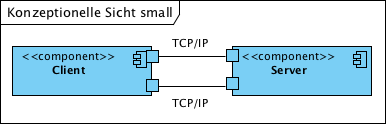
\includegraphics[scale=2]{Diagramme/KonzeptionelleSichtKlein.png} 
	\label{pic:konzeptionellesichtklein} 
\end{figure}

Unsere Architektur besteht aus zwei grundlegenden Komponenten, der Serverkomponente und der Clientkomponente (siehe Abb. \vref{pic:konzeptionellesichtklein} und Abb. \vref{pic:konzeptionellesicht}). Diese Komponenten beinhalten wiederum weitere Komponenten. Auf der einen Seite haben wir unsere Serverkomponente, die alle benötigten Daten der Medien, der Nutzer und der Ausleihvorgänge der Bibliothek speichert.

Auf der anderen Seite, der Clientkomponente, muss zwischen zwei Komponenten unterschieden werden. Einmal der Komponente GUI-Client, welche sich in erster Linie an die Bibliothekare richtet und dann noch der mobile Android-Client, der sich ausschließlich an die Leser/Nutzer richtet.

Der GUI-Client stellt für die Bibliothekare alle benötigten Funktionen bereit, um eine Bibliothek zu verwalten. Der Android-Client ermöglicht dem Leser, sich Mediendetails, den Ausleihstatus einzelner Medien, seine persönliche Ausleihhistorie sowie persönliche Daten anzeigen zu lassen. Des Weiteren kann der Leser sich mittels der App Bücher zur Ausleihe vormerken und Informationen über die Bibliothek abrufen.

\begin{figure} [H] 
\caption{Konzeptionelle Sicht}  \centering
	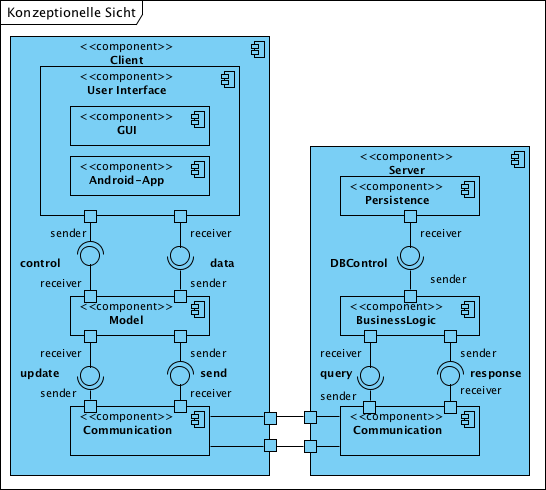
\includegraphics[width=1\textwidth]{Diagramme/KonzeptionelleSicht.png} 
	\label{pic:konzeptionellesicht} 
\end{figure}

{\centering Als Architekturstil verwenden wir das Model-View-Controller-Pattern.\\}

\subsection{Serverkomponente}
\label{sec:server}

\begin{figure} [H] 
\caption{Konzeptionelle Sicht Server}  \centering
	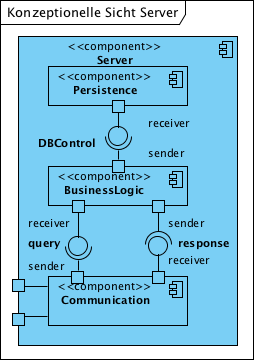
\includegraphics[scale=1.85]{Diagramme/KonzeptionelleSichtServer.png} 
	\label{pic:konzeptionellesichtserver} 
\end{figure}

Die Serverkomponente (siehe Abb. \vref{pic:konzeptionellesichtserver} besteht aus insgesamt drei Teilkomponenten, welche sich wie folgt aufgliedern:

\begin{itemize}
\item{Communication}

Die Komponente \texttt{Communication} nimmt Anfragen des Clients entgegen und leitet sie an die Komponente \texttt{BusinessLogic} weiter, wo die Anfragen verarbeitet werden und sendet die Ergebnisse zurück an den Client.

\item{BusinessLogic}

Die Komponente \texttt{BusinessLogic} dient zum Verarbeiten der Anfragen und leitet diese verarbeiteten Anfragen dann an die Komponente \texttt{Persistence} weiter.

\item{Persistence}

Die Komponente \texttt{Persistence} ist die Schnittstelle zur Datenbank. Über das Interface \texttt{DBControl} werden die verarbeiteten Anfragen von der Komponente \texttt{BusinessLogic} empfangen und in Datenbankabfragen umgewandelt, welche dann von der Datenbank entgegen genommen werden.

\end{itemize}

\subsection{Clientkomponente}
\label{sec:client}

\begin{figure} [H] 
\caption{Konzeptionelle Sicht Client}  \centering
	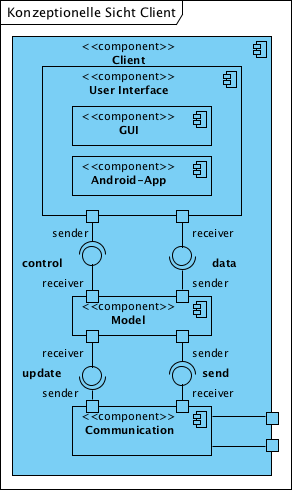
\includegraphics[scale=2]{Diagramme/KonzeptionelleSichtClient.png} 
	\label{pic:konzeptionellesichtclient} 
\end{figure}

Die Clientkomponente (siehe Abb. \vref{pic:konzeptionellesichtclient} besteht so wie die Serverkomponente aus drei Teilkomponenten, welche sich wie folgt aufgliedern:

\begin{itemize}
\item{Communication}

Die Komponente \texttt{Communication} sendet Anfragen des Clients an den Server, welche dort verarbeitet werden und nimmt die Ergebnisse entgegen, um diese an die Komponente \texttt{Model} zu übergeben, wo die Ergebnisse der Anfrage weiter verarbeitet werden.

\item{Model}

Die Komponente \texttt{Model} nimmt Ergebnisse von der Komponente \texttt{Communication} entgegen und schickt diese an die Komponente \texttt{User Interface}. 

\item{User Interface}

Die Komponente \texttt{User Interface} muss in zwei unterschiedliche Komponenten zerlegt werden:
\begin{itemize}
\item{GUI}

Die GUI richtet sich in erster Linie an Bibliothekare und nimmt alle möglichen Aktionen der Bibliothekare entgegen und schickt diese an die Komponente Model um weiter verarbeitet zu werden. Sie bildet ebenfalls eine eigenständige Komponente.

\item{Android-App}

Die Android-App richtet sich auschließlich an die Nutzer/Leser. und bietet ihnen grundlegende Funktionen die in der Anforderungsspezifikation erarbeitet wurden. Zu diesen gehören z.B. das Vormerken zur Ausleihe von Medien, Informationen über die Bibliothek anzeigen lassen, Bücher details aufrufen und seine eigenen Daten, sowie Vormerkungen und die Ausleihhistorie anzeigen lassen.

\end{itemize}

\end{itemize}

\newpage

\section{Modulsicht (Patrick, Tobias)}
\label{sec:modulsicht}

\subsection{Pakete (Patrick)}
\label{sec:pakete}

Wir haben ein Hauptpaket \texttt{eu.it\_r3v} (siehe Abb. \vref{pic:PackageUebersicht} Übersicht), in dem sich weitere Unterpakete befinden. Dies dient der Übersicht indem wir gemeinsame Quellcodedateien bündeln und so logisch zusammenhängende Einheiten erzeugen.

\begin{figure} [H] 
\caption{Pakete Übersicht} \centering
	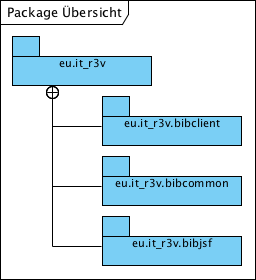
\includegraphics[scale=1.55]{Diagramme/PackageUebersicht.png} 
	\label{pic:PackageUebersicht} 
\end{figure}
\label{sec:PackageUebersicht}

\subsubsection{Paket \texttt{bibclient}}
\label{sec:bibclient}


Das Paket \texttt{bibclient}(siehe Abb. \vref{pic:PackageClient}) bündelt die Quellcodedateien die für die Android-App benutzt werden. Es besteht aus mehreren Klassen:
\begin{itemize}

\item{AsyncMediumTask.java}

AsyncMediumTask ist ein eigener AsynTask für ListMediumActivity zum holen und anzeigen der Medien.

\item{MediumAdapter.java}

Ist ein Array-Adapter und ersetzt den normalen Array-Adapter damit wir selber bestimmen können wie wir den Text aus einem Medium ziehen und ihn anzeigen lassen können.

\newpage
\item{MainActivity}

Ist der Startscreen der angezeigt wird wenn die App auf dem Smartphone gestartet wurde und geladen ist. Von hier aus erreicht man alle anderen Funktionen der App.

\item{ListMediumActivity.java}

Aktivität um die Medien in einer Liste anzeigen zu lassen.

\item{Network.java}

Die Network-Klasse sorgt für die Kommunikation der App mit dem zugehörigen REST-Service.

\item{ShowMediumActivity.java}

Die ShowMediumActivity-Klasse wird benutzt um die Detailansicht eines Mediums aufzurufen

\item{ShowUserInfoActivity.java}

Mit der Klasse ShowUserInfoActivity kann sich der Nutzer seine persönlichen Daten anzeigen lassen.

\item{LoginActivity.java}

Die LoginActivity-Klasse dient zum anmelden im System um zusätzliche Funktionen zu aktivieren, welche nur registrierten Nutzern vorbehalten sind.

\item{ShowImpressumActivity.java}

Die Klasse ShowImpressumActivity zeigt alle Information rund um die Bibliothek der Oberschule Rockwinkel an. Diese beinhalten Kontaktdaten sowie Öffnungszeiten.

\item{ShowLeasedMediumActivity.java}

Die ShowLeasedMediumActivity-Klasse zeigt alle Medien an, welche sich zur Zeit in der persönlichen Ausleige befinden.

\item{EarmarkActivity.java}

Die Klasse EarmarkActivity dient dem Vormerken von Medien zur Ausleihe.

\end{itemize}

\newpage

An weiteren Funktionalitäten der Klassen aus dem Paket \texttt{bibclient} sind noch \texttt{java.lang},
\texttt{java.util}, \texttt{java.io}, \texttt{javax}, \texttt{android}, \texttt{com.google.gson} -- eine Java-Bibliothek zum konvertieren von Java-Objekten in ihre JSON Repräsentation, \texttt{org.apache.http} -- die Kern-Interfaces und Klassen für HTTP-Komponenten, sowie \texttt{eu.it\_r3v.bibcommon.Book} zu nennen.

\begin{figure} [H] 
\caption{Paket \texttt{bibclient}} \centering
	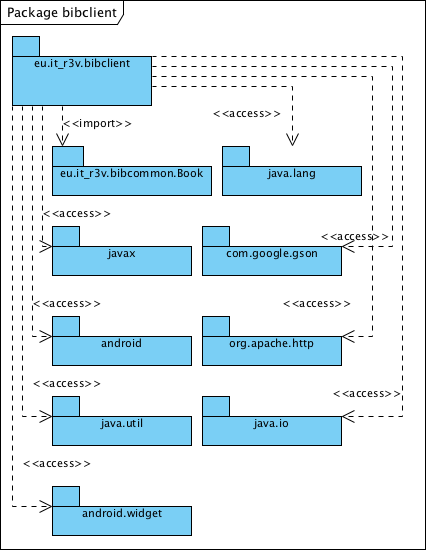
\includegraphics[scale=1.9]{Diagramme/Packagebibclient.png} 
	\label{pic:PackageClient} 
\end{figure}


\subsubsection{Paket \texttt{bibcommon}}
\label{sec:bibcommon}

Das Paket \texttt{bibcommon} stellt eine Sammlung von Quellcodedateien zur Verfügung, welche von den Komponenten \texttt{bibclient} und \texttt{bibjsf} gemeinsam genutzt werden. \texttt{bibcommon} besteht aus folgenden Klassen:

\begin{itemize}
\item{BusinessObject.java}
\item{GsonMessageHandler.java}
\item{IllegalRating.java}
\item{Reader.java}
\item{Librarian.java}
\item{Admin.java}
\item{Medium.java}
\item{Book.java}
\item{Magazine.java}
\item{Software.java}
\item{Hörbücher.java}
\item{Movie.java}
\item{CD.java}
\item{Misc.java}
\end{itemize}

Weiter Funktionalitäten auf die die Java-Klassen aus dem Paket \texttt{bibcommon} zugreifen sind \texttt{com.google.gson} -- eine Java-Bibliothek zum konvertieren von Java-Objekten in ihre JSON Repräsentation, \texttt{java.io.Serializable} -- um Klassen serialisierbar zu machen, \texttt{java.lang}, \texttt{java.util}, \texttt{java.text}, \texttt{java.ws.rs} -- High-Level-Interfaces die genutzt werden um RESTful Service-Ressourcen, was aus dem Diagramm \vref{pic:PackageCommon} ersichtlich wird.

\begin{figure} [H] 
\caption{Paket \texttt{bibcommon}} \centering
 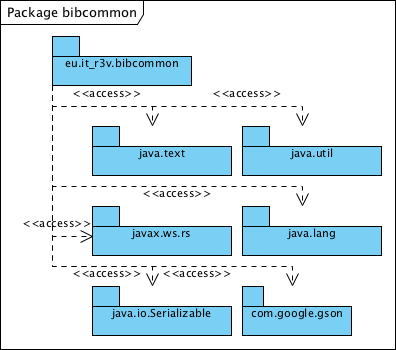
\includegraphics[scale=2]{Diagramme/Packagebibcommon.png} 
 \label{pic:PackageCommon} 
\end{figure}


\newpage
\subsubsection{Paket \texttt{bibjsf}}
\label{sec:bibclient}

Das Paket \texttt{bibjsf} besteht aus unterschiedlichen Paketen (siehe Abb. \vref{pic:Packagebibjsf}). Diese wiederum beinhalten die logisch zusammenhängenden Java-Quellcodedateien die für den Server benötigt werden. Im folgenden werden die einzelnen Pakete und die zughörigen Java-Klassen aufgelistet. 

\begin{itemize}
\item{Paket \texttt{eu.it\_r3v.businesslogic}}

\begin{itemize}
\item{BusinessHandler.java}
\item{AdministrationHandler.java}
\item{InputException.java}
\item{BusinessObjectHandler.java}
\item{ReaderHandler.java}
\item{LibrarianHandle.javar}
\item{MediumHandler.java}
\item{BorrowHandler.java}
\end{itemize}

\item{Paket \texttt{eu.it\_r3v.exceptions}}

\begin{itemize}
\item{BibJSFException.java}
\item{BookAlreadyExistsException.java}
\item{BusinessElementAlreadyExistsException.java}
\item{NoSearchBookExistException.java}
\item{DataSourceException.java}
\end{itemize}

\item{Paket \texttt{eu.it\_r3v.isbnsearch}}

\begin{itemize}
\item{GoogleAPIKey.java}
\item{ISBNGoogleSearch.java}
\end{itemize}

\item{Paket \texttt{eu.it\_r3v.persistence}}
\begin{itemize}
\item{Data.java}
\item{Persitence.java}
\end{itemize}

\item{Paket \texttt{eu.it\_r3v.presentation}}
\begin{itemize}
\item{Administration.java}
\item{AuthBackingBean.java}
\item{BusinessObjectForm.java}
\item{MediumForm.java}
\item{AddMediumForm.java}
\item{ChangeMediumForm.java}
\item{BookListDataModel.java}
\item{ReaderForm.java}
\item{AddReaderForm.java}
\item{ChangeReaderForm.java}
\item{LibrarianForm.java}
\item{AddLibrarianFrom.java}
\item{ChangeLibrarianForm.java}
\item{TableDataModel.java.java}
\item{TableForm.java}
\item{MediumTable.java}
\item{ReaderTable.java}
\end{itemize}

\item{Paket \texttt{eu.it\_r3v.renderer}}

\begin{itemize}
\item{Content.java}
\item{IDCardPrinter.java}
\item{IDContent.java}
\item{Printer.java}
\item{MediumTagPrinter.java}
\item{MediumTagContent.java}
\end{itemize}

\item{Paket \texttt{eu.it\_r3v.services}}

\begin{itemize}
\item{Bibservices.java}
\end{itemize}

\item{Paket \texttt{eu.it\_r3v.utils}}

\begin{itemize}
\item{Configuration.java}
\item{Constraint.java}
\item{CSVReader.java}
\item{EqualConstraint.java}
\item{LikeConstraint.java}
\item{Messages.java}
\item{OrderBy.java}
\item{Reflection.java}
\end{itemize}

\end{itemize}


\begin{figure} [H] 
\caption{Paketübersicht \texttt{bibjsf}} \centering
 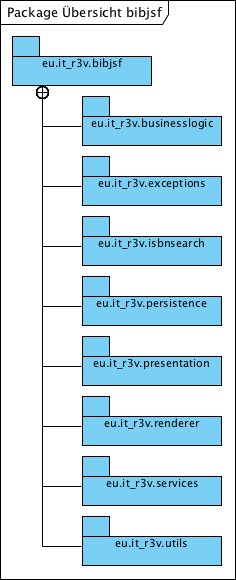
\includegraphics[width=0.45\textwidth]{Diagramme/Packagebibjsfuebersicht.png} 
 \label{pic:Packagebibjsf} 
\end{figure}

Der Abb. \vref{pic:PackagebibjsfUebersicht} sind die weiteren Funktionalitäten \texttt{org.primfaces} -- eine Open-Source JSF Komponentensammlung mit unterschiedlichen Erweiterungen), \texttt{com.google.api} -- eine Bibliothek für Zugriff auf Googe APIs via JSON, \texttt{eu.it\_r3v.bibjsf}, \texttt{eu.it\_r3v.bibcommon}, \texttt{org.apache} -- die Kern-Interfaces und Klassen für HTTP-Komponenten, \texttt{javax}, \texttt{java.text}, \texttt{java.sql} -- für den Zugriff auf Datenbank, \texttt{java.security} -- eine Sammlung von APIs und Tools zur Implementierung von Sicherheitsalgorithmen, \texttt{java.util}, \texttt{java.math}, \texttt{java.lang} und \texttt{java.io} zu entnehmen, welche von den einzelnen Java-Klassen benötigt werden.


\begin{figure} [H] 
\caption{Paket bibjsf} \centering
 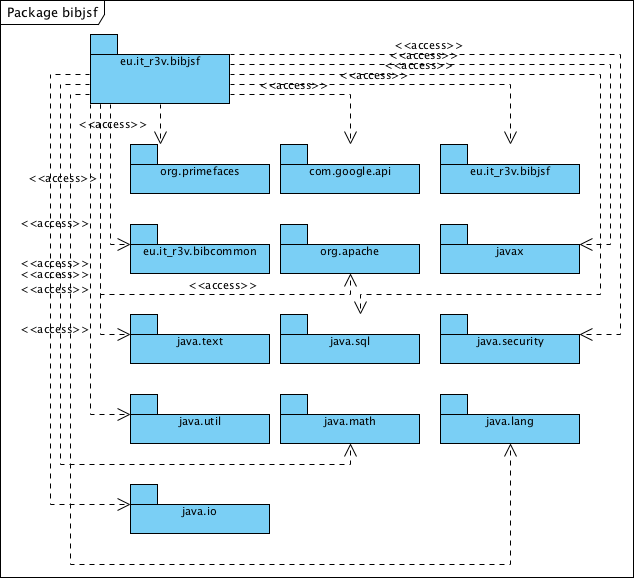
\includegraphics[width=1\textwidth]{Diagramme/Packagebibjsf.png} 
 \label{pic:PackagebibjsfUebersicht} 
\end{figure}

\newpage

\subsection{Klassendiagramme (Tobias)}

Im Folgenden werden die einzelnen Pakete in Klassendiagramme umgestellt, da 
ein einzelnes Klassendiagramm aller benutzten Klassen unübersichtlich wäre.
Zusätzlich sei angemerkt, dass die Klassen lediglich mit Methoden oder Attributen.
angezeigt werden, sofern sie durch die Projektarbeit neu erstellt oder verändert wurden.
Außerdem sei noch angemerkt, dass sich zwar Änderungen z.B. von Variablen durch die Erweiterung der Mindestanforderungen ergeben. Diese kleinen Änderungen werden aber im Folgenden nicht berücksichtigt.
\newpage

\subsubsection{Klassendiagramme \texttt{bibjsf}}

\textbf{BusinessLogic:}

Das Package \texttt{BusinessLogic} erhält hinzukommend \texttt{LibrarianHandler}. Die Klasse
\texttt{BookHandler} wird durch \texttt{MediumHandler} ersetzt.
\texttt{LibrarianHandler} erhält die Methoden:
\texttt{addLibrarian()},
\texttt{deleteLibrarian()},
\texttt{editLibrarian()}. \\
\texttt{MediumHandler} erhält dieselben Methoden wie \texttt{BookHandler}, nur dass die Methodennamen 
mit dem Namensinhalt \texttt{Book} in \texttt{Medium} geändert werden. Zum Beispiel:
\texttt{getAllBooks():List<Book>} wird zu  \texttt{getAllMedien():List<Medium>}. Diese Veränderungen haben den Zweck, \texttt{MediumHandler} für alle Medientypen verwenden zu können, wofür zutreffendere Methodennamen geeigneter sind:
\texttt{getAllMedien()},
\texttt{add(Medium)},
\texttt{update(Medium)},
\texttt{delete(List<Medium>)}.

\begin{figure} [H] 
\caption{Paket \texttt{BusinessLogic}} \centering
 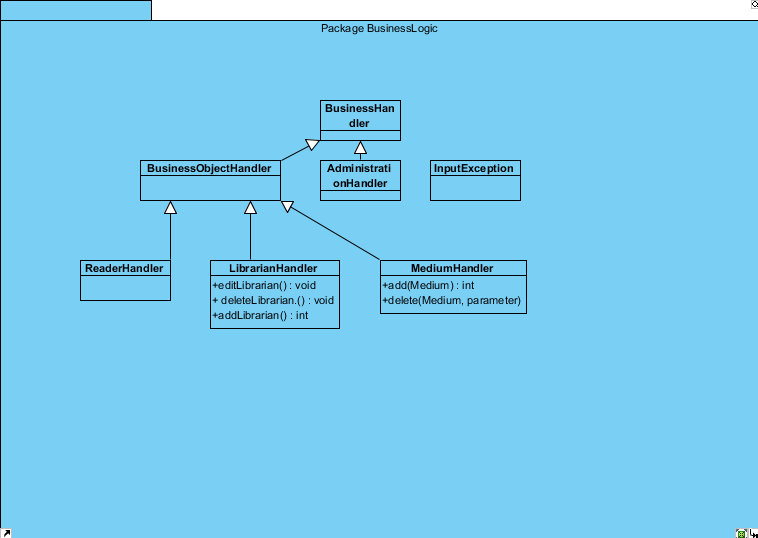
\includegraphics[width=1\textwidth]{Diagramme/BusinessLogic.png} 
 \label{BusinessLogic} 
\end{figure}

\textbf{Presentation:}

Die ehemaligen Klassen \texttt{BookForm, AddBookForm} und \texttt{ChangeBookForm} werden durch \texttt{MediumForm}, \texttt{AddMediumForm} und \texttt{ChangeMediumForm} ersetzt. Die Oberklassen \texttt{ReaderForm} und \texttt{LibrarianForm} werden hier vorerst nicht unterschieden. Die Klasse \texttt{MediumForm} unterscheidet sich, abgesehen von dem Namen, nicht von der ehemaligen Klasse \texttt{BookForm}. Es werden hier also keine weiteren Methoden eingesetzt, die nicht schon in den ehemaligen Klassen vorhanden waren.

\begin{figure} [H] 
\caption{Paket \texttt{Presentation}} \centering
 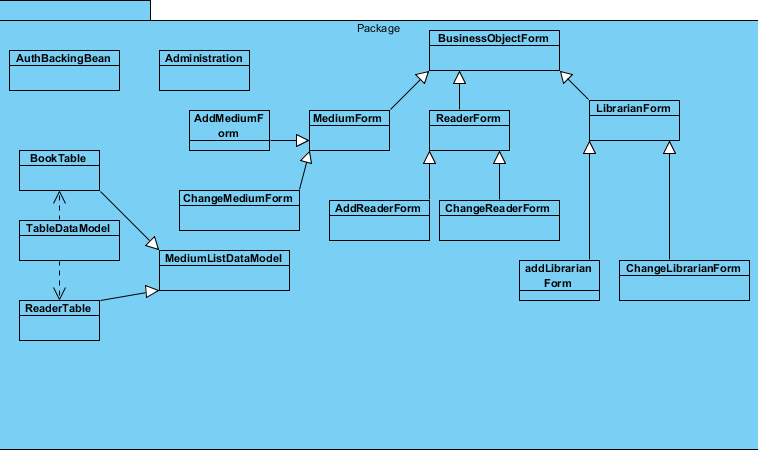
\includegraphics[width=1\textwidth]{Diagramme/Presentation.png} 
 \label{Presentation} 
\end{figure}

\textbf{Persistence:}

Im Paket \texttt{Persistence} kam es bisher zu keinen erwähnenswerten, signifikanten Änderungen oder Erweiterungen in Form von Methoden o.Ä.

\begin{figure} [H] 
\caption{Paket \texttt{Persistence}} \centering
 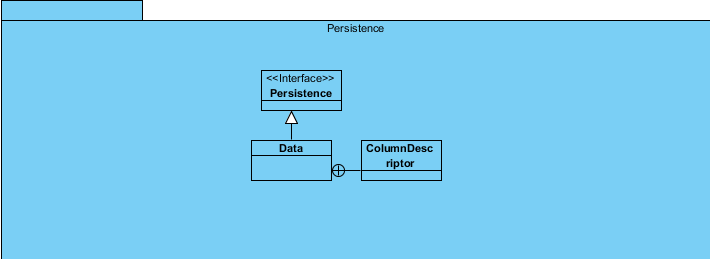
\includegraphics[width=0.9\textwidth]{Diagramme/Persistence.png} 
 \label{Persistence} 
\end{figure}
\newpage

\textbf{Renderer:}

Da wir nun die Klassen \texttt{MediumTagPrinter} und \texttt{MediumTagContent} haben, unterstützt das Package nun mehrere Medien und nicht nur Bücher, so wie es zuvor implementiert war.
\begin{figure} [H] 
\caption{Paket \texttt{Renderer}} \centering
 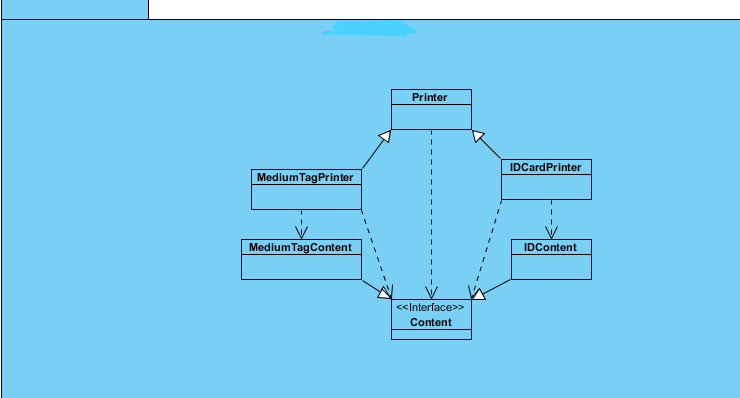
\includegraphics[width=0.9\textwidth]{Diagramme/Renderer.png} 
 \label{Renderer} 
\end{figure}

\textbf{Utils:}

In diesem Paket wurde bisher nichts erweitert, was wir für angemessen hielten.
\begin{figure} [H] 
\caption{Paket \texttt{Utils}} \centering
 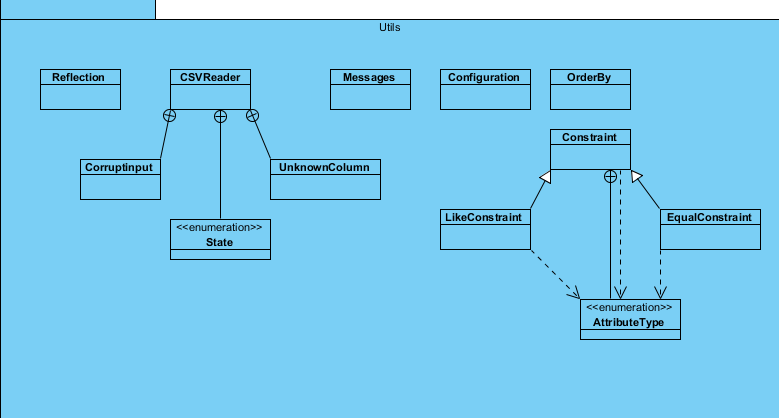
\includegraphics[width=0.8\textwidth]{Diagramme/Utils.png} 
 \label{Utils} 
\end{figure}
\newpage
\textbf{Exception:} \\
In diesem Paket haben wir bisher die Klassen, die mit Büchern arbeiten, noch nicht in entsprechende Klassen für Medien, wie z.B. \texttt{MediumAlreadyExists} geändert, weil wir dies zu diesem Zeitpunkt noch nicht für erforderlich hielten.
\begin{figure} [H] 
\caption{Paket \texttt{Exception}} \centering
 \includegraphics[width=1\textwidth]{Diagramme/exception.png} 
 \label{Exception} 
\end{figure}

\textbf{ISBNSearch:}
In diesem Paket wurde bisher nichts erweitert, was wir für angemessen hielten.
\begin{figure} [H] 
\caption{Paket \texttt{ISBNSearch}} \centering
 \includegraphics[width=0.7\textwidth]{Diagramme/ISBNSearch.png} 
 \label{ISBNSearch} 
\end{figure}

\textbf{Services:}
In diesem Paket wurde bisher nichts erweitert, was wir für angemessen hielten.
\begin{figure} [H] 
\caption{Paket \texttt{Services}} \centering
 \includegraphics[width=0.7\textwidth]{Diagramme/services.png} 
 \label{Services} 
\end{figure}


\subsubsection{Klassendiagramm \texttt{BibClient}}
In diesem Paket haben wir keine Veränderungen implementiert.
\begin{figure} [H] 
\caption{Paket \texttt{BibClient}} \centering
 \includegraphics[width=0.8\textwidth]{Diagramme/bibclient.png} 
 \label{BibClient} 
\end{figure}

\subsubsection{Klassendiagramm \texttt{BibCommon}}
Hier haben wir die größten Änderungen vorgenommen. Wir haben nämlich Unterklassen von \texttt{Medium} implementiert, die entsprechend davon erben, wie \texttt{Book, CD, Hörbücher} usw. mit entsprechenden Attributen, die nur auf das entsprechende Medium zugeschnitten sind.
\begin{figure} [H] 
\caption{Paket \texttt{BibCommon}} \centering
 \includegraphics[width=0.8\textwidth]{Diagramme/bibcommon.png} 
 \label{BibCommon} 
\end{figure}


\section{Datensicht (Tobias)}
\label{sec:datensicht}

\begin{figure} [H] 
\caption{Paket \texttt{BibCommon}} \centering
 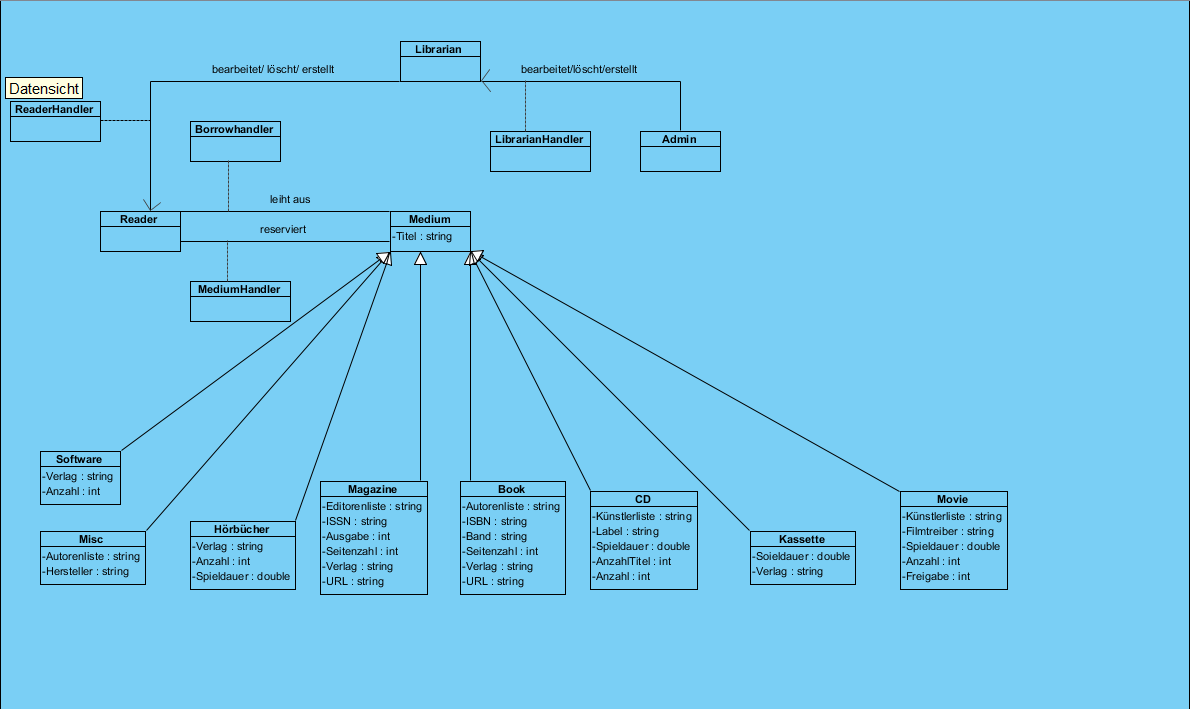
\includegraphics[width=0.8\textwidth]{Diagramme/Datensicht.png} 
 \label{BibCommon} 
\end{figure}

Veränderungen: Die einzelnen Personen( Admin, Librarian und Reader) leiten sich nicht mehr von Person ab, da diese nicht vom Datenmodell übernommen wurde. Bibliothekar heißt nun Librarian. 
Die Klassen Bewertung und Rezensieren wurden ebenfalls entfernt, da sie sich nicht mehr innerhalb unserer Mindestanforderungen befinden. Das Bearbeiten von Personen also entweder Librarian oder Reader wird mit den Handler-Klassen geregelt.\\

\section{Ausführungssicht (Sebastian)}

Das folgende Diagramm \vref{ausfuehrungssicht} zeigt das Laufzeitverhalten der Software.
Auf der einen Seite haben wir den mobilen Zugang, auf dem die Android App als Prozess läuft. Die App selbst verwendet die Module \texttt{bibclient} und \texttt{bibcommon}. Von diesem mobilem Zugang kann eine TCP/IP-Verbindung zu dem Bibliotheksserver aufgebaut werden. Dabei gibt es mehrere Verbindungen zu immer nur einem Server, daher die Multiplizitäten \texttt{*} und \texttt{1}.

Auf der anderen Seite nimmt nun der Bibliotheksserver die TCP/IP-Verbindungen an. Er ist gleichzeitig Server und Datenbankserver. Die Datenbank läuft auf dem Subsystem Glassfish Server. Der Server verwendet die Module \texttt{businesslogic, exception, isbnsearch, persistence, presentation, properties, renderer, services} und \texttt{util}.

Das komplette System läuft mit zwei Prozessen: einmal mit der Android App und dem anderen Prozess \texttt{bibjsf}, der das Subsystem mit der Datenbank enthält. Prinzipiell gibt es unendlich viele mobile Zugänge bzw. App-Prozesse, die auf einen Bibliotheksserver zugreifen.

\begin{figure} [H] 
\caption{Ausführungssicht} 
	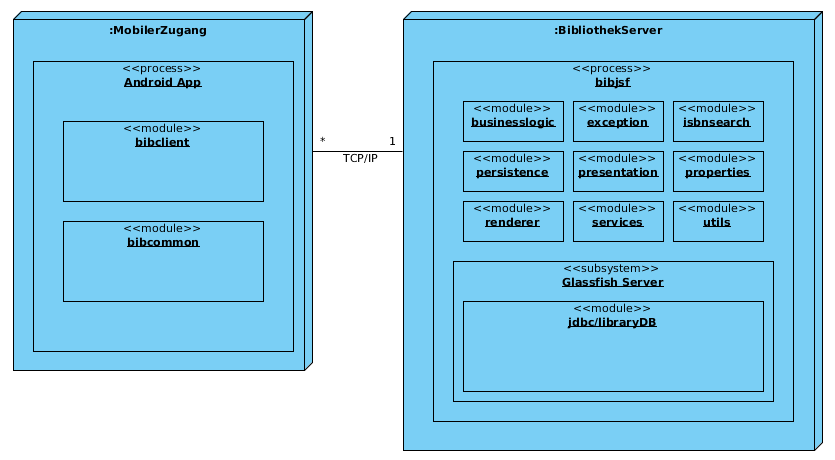
\includegraphics[width=1\textwidth]{Diagramme/ausfuehrungssicht.png} 
	\label{ausfuehrungssicht} 
\end{figure}
\label{sec:ausfuehrung}

\section{Zusammenhänge zwischen Anwendungsfällen und Architektur (Tim)}
\label{sec:anwendungsfaelle}



\section{Evolution (Tim)}


\label{sec:evolution}

In diesem Abschnitt geht es um mögliche Änderungen, Anpassungen bzw. Erweiterungen, die vorgenommen werden müssten, wenn sich Anforderungen des Systems ändern. \\
Dabei ist wichtig, dass sich solche Änderungen möglichst modular realisieren lassen, ohne die bestehende Architektur komplett zu verändern, was sehr aufwändig und somit nicht wünschenswert wäre. \\
Im Folgenden werden einige wichtige mögliche neue Anforderungen bzw. Erweiterungen aufgelistet und deren jeweiligen zu implementierenden Änderungen an der Architektur beschrieben. 

\subsection*{Erweiterungsmöglichkeiten aus der Anforderungsspezifikation}

Wir haben bereits in der Anforderungsspezifikation im Punkt ''Ausblick'' zwei mögliche Änderungen genannt, die wir im hier detaillierter beschreiben möchten. 

\subsubsection*{1. Medientypenzuwachs}

Wie schon in der Anforderungsspezifikation im Punkt ''2.7 Ausblick'' angedeutet, wäre eine zu erwartende bzw. recht wahrscheinliche Erweiterung der Bibliothekssoftware, neben den vorhandenen Medien wie Büchern, Zeitschriften, CDs usw. weitere Medien wie z.B. Blu-Rays verwenden zu wollen und diese entsprechend im System aufzunehmen.\\
Da in unserem System nicht alle Medien allein für sich stehen, sondern ihre gemeinsamen Eigenschaften ihrer Klassen in einer Superklasse namens \texttt{Medium} zusammengefasst werden, ist es recht einfach, einen solchen Medientypenzuwachs ohne großen Aufwand zu realisieren. Man muss lediglich eine weitere Subklasse der Klasse \texttt{Medium}, z.B. mit Namen \texttt{BluRay} ins Modul \texttt{bibcommon} einbauen.

\subsubsection*{2. Erweiterung des Systems für iOS-Geräte}

Wir werden für unser System eine Android-App entwickeln, die für den mobilen Zugang mit Smartphones einen Zugang zu dem Bibliothekssystem bietet. Da Android sehr verbreitet ist, werden wir mit dieser Lösung sicherlich viele Nutzer erreichen können, jedoch natürlich längst nicht alle. \\
Insofern wäre zu überlegen, ob man nicht auch eine zusätzliche App für iOS-Geräte entwickeln könnte. Um dies zu realisieren, bedarf es jedoch nicht, wie oben angestrebt, modularen Änderungen, sondern der Entwicklung eines grundlegend anderen Systems. Insofern kann an dieser Stelle auch nicht beschrieben werden, welche Änderungen vorzunehmen sind, weil es sich hierbei ja eben nicht um aufbauende Erweiterungen des bestehenden Systems, sondern im Prinzip um eine Neuentwicklung einer zweiten App handeln  würde.

\subsection*{Zusätzliche denkbare Erweiterungen}

Über die genannten Punkte aus der Anforderungsspezifikation hinaus könnten sich weitere Änderungen ergeben, die im Folgenden beschrieben werden.

\subsubsection*{1. Erweiterung des GUI-Layouts}

Es wäre möglicherweise durchaus wünschenswert, wenn man als Benutzer nicht nur ein GUI-Design verwenden könnte, sondern mehrere. Dafür müsste eine Funktionalität hinzugefügt werden, um zwischen verschiedenen Benutzeroberflächen wählen zu können. \\
Dazu müssten entsprechende Referenzierungen von neuen GUI-Style-Änderungen mit Bilddateien stattfinden sowie für Textanpassungen die XML-Dateien im Paket \texttt{biblient/res/layout} verändert bzw. erweitert werden. 

\subsubsection*{2. Mehrsprachigkeit}

Gemäß den Mindestanforderungen wird das System so implementiert sein, dass die Möglichkeit besteht, mehrere Sprachen für das Bibliothekssystem zu unterstützen. Insofern wäre es denkbar, dass neben Deutsch eine weitere Sprache eingebaut werden könnte. Englisch würde sich natürlich anbieten.
\end{document}